%2345678901234567890123456789012345678901234567890123456789012345678901
%\newcommand{\classname}[1]{\textsc{#1}}

% chapter radams (fold)
\chapter[Radio Astronomical DAta Model for Single-dish radio
telescopes]
{RADAMS: a Radio Astronomical DAta Model for Single-dish radio
telescopes}
\label{cha:radams}
	
	In the past chapters we have been making emphasis on how the VO
	works by providing common data access protocols, common data
	formats for information interchange, and a common data model
	for expressing, within the constraints of the data model and
	data access protocols of the VO, the description of
	observational data.
	
	In particular, in the previous chapter we have shown the
	general framework proposed by the IVOA for describing whole
	observations, characterising the parameter space occupied by
	them, and using a specific format/data model for indicating
	space and time restrictions. We have also seen that the
	Observation data model is not complete, while the CharDM and
	STC are mature enough to have been granted the IVOA
	Recommendation status. However, they have never been applied to
	radio astronomical archives, and have never been used as the
	basis for a radio astronomical archive.
	
	In this chapter we will try to answer the question: \emph{How
	to architecture a VO-compatible radio astronomical archive?},
	and for that we will use the outlined ObsDM as a foundation in
	order to create a complete data model for radio astronomical
	observations which can be used both for the development of
	single-dish radio astronomical archives, enhancing the existing
	IVOA Observation data model at the same time.
	
	\section{Basic requirements of astronomical archives} % (fold)
	\label{sec:radams_archive_basics}
		
		We will start stating the obvious: a radio astronomical
		online archive has to provide a way for astronomers to find
		and retrieve radio astronomical observations. The most
		simple incarnation of such an archive would include a
		complete list of all observation files, together with a
		system for retrieving the actual file containing the
		observational data set.
		
		With such a simple archive system only people aware of what
		was observed and contained in each file would be able to use
		it. Thus, the most basic additional requirement all
		astronomers would need is coordinate searching, or the
		ability to identify files with positions in the celestial
		sphere.
		
		The next requirement in order of importance is the
		identification of the band of the electromagnetic spectrum
		being scanned by the instrument, \invisiblenote{when
		different bands are observable.} as different bands provide
		diverse information on the physical processes taking place
		in the observed region. This is the first place where the
		specifics of radio astronomy begin to emerge.
		
		These pieces of information  do not actually belong
		to the science data themselves, and are metadata for the
		observation. In particular, the two examples above can be
		identified to the lowest levels of detail in the CharDM
		for the spatial and spectral axes (Location and Bounds in
		both axes).
		
		This small example tells us two things: first, it shows
		that the most important metadata needed for information
		filtering are already part of the proposed IVOA data models;
		and second, that such data models can be used as a
		blueprint for astronomical archives
		
		\begin{figure}[tbp]
			\centering
			
			\subfloat[][]
			{
				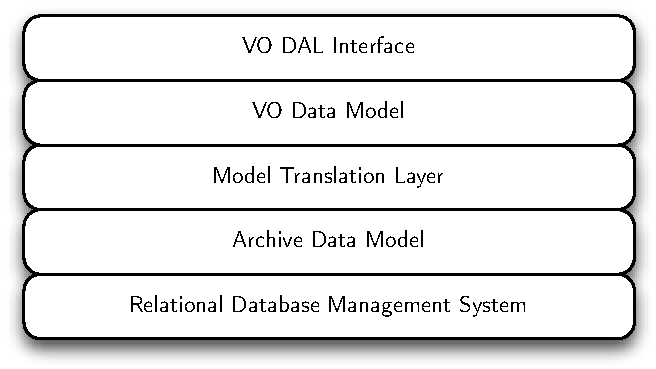
\includegraphics[width=0.47\columnwidth]
				{fig/VODalArchiveLayers.pdf}
				\label{subfig:fig_VODalArchiveLayers}
			} 
			\hfill 
			\subfloat[][]
			{
				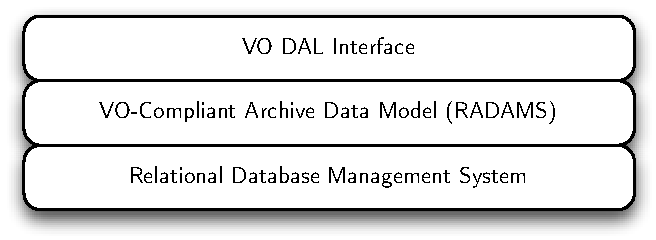
\includegraphics[width=0.47\columnwidth]
				{fig/VORadamsLayers.pdf}
				\label{subfig:fig_VORadamsLayers}
			} 
			\caption[Data modelling layers for different kinds of VO
			archives]
			{
				Data modelling layers for different kinds of VO
				archives. Subfigure
				\subref{subfig:fig_VODalArchiveLayers} shows the
				layered structure of a VO archive built on an
				existing, while~\subref{subfig:fig_VORadamsLayers}
				shows the simplicity of an archive built from
				scratch for VO compatibility.
			}
			\label{fig:VODalRadamsArchiveLayers}
		\end{figure}
		
		A welcome side-effect of directly using VO data 
		models as the basis for astronomical archives is that
		their use simplifies the archival development, and the
		integration of fully described archives in the VO.
		
		To illustrate this,  we will compare the
		development layers and complexity needed to build VO
		compatibility both on existing archival systems, and 
		by building an archive from scratch.
		Figure~\ref{fig:VODalRadamsArchiveLayers} shows both
		kinds of archives side by side.
		
		In the case of an archive with an already existing
		infrastructure
		---sub\-fi\-gu\-re~\ref{subfig:fig_VODalArchiveLayers}---,
		VO data models have to be mapped on top of a translation
		layer in charge of creating VO entities from the existing
		archive data model. But if the archive is going to be built
		from scratch, the Data Access Layer (DAL)
		interfaces\footnote{The DAL data model and interface will
		be briefly described in relation with the different data
		products to be delivered.} can be built on top of the VO
		entities directly provided by the archive infrastructure
		---in the case of
		sub\-fi\-gu\-re~\ref{subfig:fig_VORadamsLayers}, the
		RADAMS---.
		
		It should be noticed that for building VO archives on top
		of an existing, non-VO archive, the translation layer has
		to provide some metadata which do not only need
		translation, but in many cases those metadata have to be
		extracted or even calculated from either the FITS headers,
		the actual FITS data tables/images, or even the observation
		logs\footnote{Possibly, even a combination of all of
		them. Actual examples will be shown in the chapter devoted
		to radio astronomical characterisation with the RADAMS.}.
		
		\suppress[Enrique]{
		Not all the pieces of information needed to build the whole
		RADAMS metadata come directly from the FITS data, but
		instead come from observing logs, or as mentioned before,
		from the actual data, and might be lost if they are not
		explicitly stated. Creating a new archive conforming to
		IVOA data models ensures the availability of the data
		sources for the VO metadata, and allows for an ideally
		direct translation between the archive and DAL layers.}
		
	% section radams_archive_basics (end)
	
	\section{RADAMS requirements and overview} % (fold)
	\label{sec:radams_requirements_overview}
		Once established that a VO-based data model can indeed be
		used as the basic architecture for an astronomical
		archive, we can define which will be the requirements of
		such a data model for radio astronomical observations,
		our RADAMS.
		
		\begin{description}
			\item[Based on the Observation and Characterisation DMs]
			The RADAMS is a da\-ta model for the metadata regarding a
			radio astronomical single-dish observation, and as such
			is based on the Observation data model. In order to
			complete the RADAMS, extensions are provided within the
			framework of the ObsDM and the CharDM.
			
			\item[Separation of data and metadata] In a RADAMS
			based archive, data will be stored in the form of FITS
			files or VOTables, whereas all metadata will be stored
			in database form complying with the RADAMS. For already
			existing archives, this condition is relaxed, but a
			query mechanism for all RADAMS metadata should be
			available.
			
			\item[Single-feed observations] Metadata and
			observations are considered always to be referring a
			single feed. If a telescope or instrument is able to
			provide several feeds simultaneously, each one will be
			stored separately, and will refer to the same observing
			proposal, but will have a separate existence.
			
 			\item[Radio astronomical data products] The RADAMS will
 			be able to support data of the following kinds:
			
			\begin{itemize}
				\item Single-pointing flux measurements;
				
				\item Single-pointing radio astronomical spectra,
				or spectra associations;
				
				\item On-the-fly on-off, spectra data, or 
				continuum flux observations, in the form of images
				and data cubes;
			\end{itemize}
			
			The data product definition must be made compatible
			with existing IVOA DAL protocols: images (SIA protocol),
			sets of
			spectra (SSA protocol), and coordinates-based data tables.
			
		\end{description}
		
		From those requirements, we have built the RADAMS data
		model, whose high-level structure is shown in
		figure~\ref{RADAMSHLoverview}. We can see that we have
		closely followed the ObsDM, and the CharDM, and that in
		order to use 
		the whole ObsDM we will need to provide definitions for
		some of the classes.
		
		\begin{figure}[tbp]
			\begin{center}
			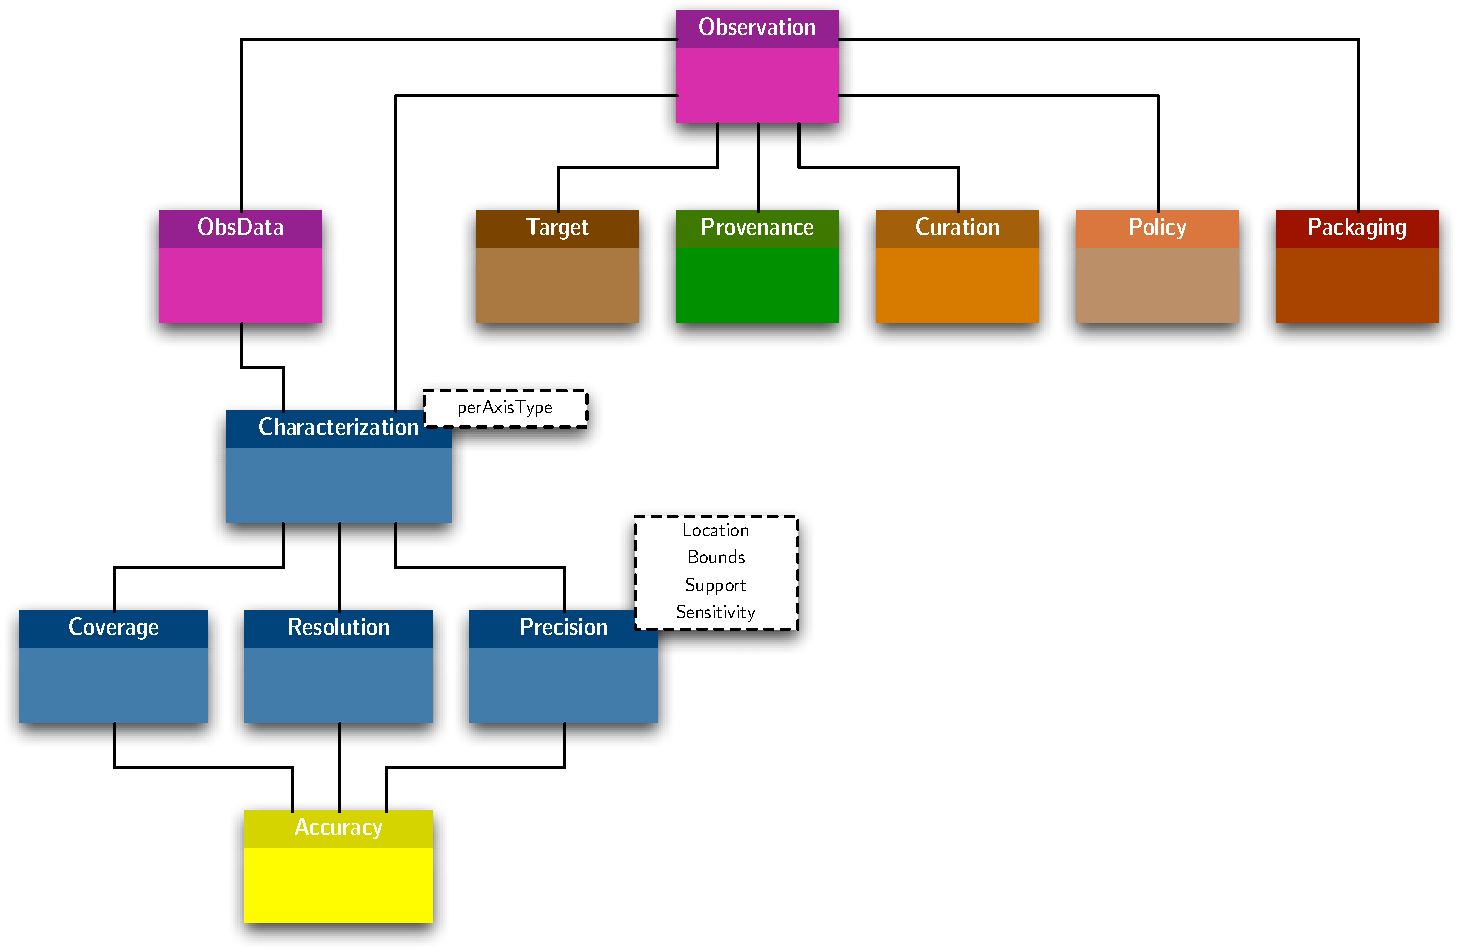
\includegraphics[width=\columnwidth]
				{fig/RADAMS_Complete}
			\caption[RADAMS general class organisation]{
				RADAMS general class organisation. Different colours
				correspond to different sub-models, and will be
				kept in the next chapters.
			}
			\label{RADAMSHLoverview}
			\end{center}
		\end{figure}
		
		Those classes and sub-models defining the RADAMS will be,
		then:
		
		\begin{description}
			\item[Observation] Root class for the data model. It
			works as a hub to which both actual observational data
			(ObsData) and the remaining metadata are linked
			together.
			
			\item[ObsData] Describes how to access the actual
			data being described by all the RADAMS' classes.
			
			\item[Target] Describes the target of the observation,
			providing as much information as available for
			already known targets.
			
			\item[Characterisation] Corresponds to the CharDM
			classes.
			
			\item[Provenance] Links all the information regarding
			the origin of the observation, both from an
			administrative, technical and scientific point of
			view.
			
			\item[Curation] Describes who is responsible for
			maintaining a particular observation, a set of
			observations, or all of the archive.
			
			\item[Policy] Is used to specify the access rights
			for different systems and persons accessing the
			archive.
			
			\item[Packaging] Describes the way an observation,
			or a set of observations, are actually delivered
			when the archive is queried.
		\end{description}
		
		We will describe these classes in the following sections,
		and we will leave their exact implementation details to
		specific chapters.
	% section radams_requirements_overview (end)

	\section{Observation and ObsData} %(fold)
	\label{sec:observation_obsdata}

		The Observation class is the root class of the data model.
		It describes an arbitrarily large dataset that can be
		derived directly from an observation, or from several
		observations. Generally, we will consider an Observation as
		the set of data recorded with the same instrumental
		setting, and with the same associated target during a
		continued period of time.

		% In the particular case of the DSS-63, an Observation would
		% be made of the set of on/off observations associated with
		% the same target, or the final, flux calibrated spectra. As
		% we will see later, the Packaging class will allow us to
		% have different degrees of granularity for data access.
		
		On the other hand, the ObsData class is a proxy class
		representing the actual data, and holding a reference that
		the archive interface can use to retrieve or provide
		science-ready data files.
		
		The Observation class, then, is used to link together
		the different aspects of the observation, from the
		originating proposal (Curation) to the reduced data
		(ObsData), and taking into account also the data
		Characterisation, the data access Policy, etc.
		
		However, a direct link is also preserved between the
		ObsData and the Characterisation, so that if data is
		repackaged the mapping to the Characterisation metadata can
		be preserved.
		
		The Observation class, then, only needs a unique identifier
		for each unique observation, what brings to the table what
		is the minimum observation (in practice, ObsData) to be
		collected by the RADAMS. We will answer that in the next
		chapter.
		
		% For sets which can be provided either as individual
		% datasets, or as joined 
		% The RADAMS makes use of the Packaging class ---which we
		% will define below--- in order to specify what particular
		% pieces of data are being retrieved. Besides, the archival
		% of continuum information cannot be discarded, as most radio
		% telescopes are capable of performing continuum scans.
				
	% section observation_obsdata (end)
	
	
	\section{Characterisation} %(fold)
		
		The Characterisation class
		provides
		the quantitative and qualitative description of the
		observational data in multiple axes. This information is
		stored conforming to the most current CharDM IVOA
		Recommendation~\cite{2008dmadcrept.....L}.
		
		As seen in the previous chapter, we can consider that any
		astronomical measurement occupies a position in a
		multi-di\-men\-sion\-al space, defined by several axes.
		Initially, this axes are just four (but more can be added):
		spatial (coordinates), temporal, spectral, and a fourth
		axis corresponding to the observed physical quantity (e.g.,
		measured flux, or polarisation, in the case of radio
		observations). Characterisation gives us a description of
		the data in different attributes and levels of detail
		inside this multi-di\-men\-sion\-al space, including
		physical units and scales.
		
		The Characterisation class for each individual axis
		can be divided in the following
		subclasses:
		
		\begin{description}
			\item[Coverage] Specifies which part of the
			multi-di\-men\-sion\-al space has been encompassed by
			the measurement. That is, when was the observation made
			and for how long, which field was covered, which bands
			were studied, what was the range of observed flux, and
			so on. Each of those questions belongs to a different
			axis.
			
			 \item[Resolution] Specifies data resolution in each of
			the axes. Resolution is independent of the sampling, as
			it is a property of the instrument/observing process.
			
			 \item[Precision] When data are sampled in any
			of the axes
			(e.g., for spectral data in the frequency domain, data
			are sampled by means of filter banks, or by FFT from 
			an autocorrelation signal),
			this class will include information on
			the sampling precision\footnote{This is different from
			resolution: resolution is a property of the instrument,
			due to uncertainties on the energy distribution of the
			source, because of convolution of the source’s and the
			instrument’s profiles.}.
			
			\item[Accuracy] Specifies the minimum error rate
			achievable for each axis, both from systematic and
			random errors.
		\end{description}
		
		From this group we can see that for Coverage, Resolution and
		Precision information can be defined
		\emph{a priori} for a whole observing program (in the
		Characterisation of a Registry entry, for instance), but they
		can be different for each actual observation dataset, and
		those will be the ones stored by the RADAMS.
		
		In contrast, Accuracy information needs to
		be evaluated \emph{a posteriori}: the lower bounds of 
		accuracy can be known from instrument calibration and
		knowledge of the observation process, but for some axes
		assessing the accuracy actually achieved needs access to
		historical information.
		
		
		
			
		%	 \item[Sensitivity] This class quantifies the
		%	sensitivity of the instrument in the given axis, by
		%	means of a sensitivity function that is defined for the
		%	whole coverage of the observation in the given axis.
		%	This class has not been fully defined yet by the IVOA
		%	Working Group, hence we are providing a tentative
		%	description of this class, in order to help the the
		%	efforts of the Characterisation Working Group.
			
		
	% section Characterisation (end)
	
	\section{Target/Field} %(fold)
	\label{sec:radams_target}
		
		As we have mentioned several times, astronomers study most
		of the time objects they already know, while other times
		they probe a certain part of the sky to see if there is
		something new, or even survey a whole region in order to 
		later exhaustively study that region and all objects they
		can find in it.
		
		This class allows the RADAMS to include information 
		about observed targets. Such target can be mapped to
		known astronomical objects, to detected sources, to a given
		field, et cetera. Having this entity in a separate class from
		the Observation one allows to perform queries by Target, and
		the ability to link external target information using VO
		services (such as Sesame, Aladin, the SkyNode interface,
		et cetera).
		
		In order to be linked with ObsData and Observation
		classes, the unique identifier for the observation is
		stored, which allows for queries on given targets to
		return observations, but also for observation sets to
		retrieve Target information.
		
	% section Target (end)
	
	\section{Provenance} %(fold)
		
		This class groups all the information describing the way
		an astronomical dataset was originated.
		It has to include the instrumental
		setting for that particular observation, coordinates for
		the telescope, weather and atmospheric conditions, and all
		the information about data pre- and post-processing,
		when such data were created by processing already existing
		datasets\footnote{This is already the case for reduced data,
		which makes extensive use of calibration information,
		background models and measurements, et cetera.}.
		
		Again, the link with ObsData is the unique observation
		identifier, but for some of the information, which are
		recorded automatically by the engineering data collection
		systems, time-stamps will need to be used to bound the
		relevant information (for instance, focus and pointing
		calibration observations).
		
	 % section Provenance (end)
	
	\section{Policy} % (fold)
		
		In astronomy, observation data are the property of the
		investigator having suggested and planned the observation,
		for a period which in some cases depends completely on the
		observer, which might decide never to release to the public
		the observations he made, and in other cases depend on
		policies implemented by the organisation providing the
		observing facility. Typical cases are 12 to 24 months of
		proprietary data from the moment the observation was
		performed to the moment the observation is made available
		to the general community.
		
		Some observatories have policies where different access
		rights are available depending on the country or the
		organisation a particular investigator belongs to, due
		to different agreements between the hosting organisation
		and data requesting parties.
		
		This class allows both for the tagging of the observation
		data, and for establishing the data access rights for 
		datasets depending on the Policy information for the 
		dataset itself, and for the user.
		
		Examples of widely different data access policies can be
		found in archives such as the European Southern Observatory
		Archive\footnote{The archive of the ESO, for instance, makes
		header information (including pointing) available
		immediately after observation, together with calibration
		data. Actual science data are only released after a
		proprietary period (which can be extended under demand),
		together with observation proposal abstracts. Their policy
		can be found at
		\url{http://archive.eso.org/cms/eso-data-access-policy}}
		(ESO). A more general view on scientific data access
		policies can be found on the Committee on Data for Science
		and Technology (CODATA) of the International Council for
		Science (ICSU) on their Scientific Data Policy Statements
	website\urlnote{http://www.codata.org/data_access/policies.html}.
		
		In order to accommodate all these different kinds of data
		access policies, we have chosen a role-based approach,
		where different permissions are allowed not to each
		different user, but regarding the role that user has
		against a particular piece of information. This mechanism
		will be discussed in detail in chapter~\ref{sec:policy}.
		
	% section Policy (end)
	
	\section{Curation} %(fold)
		
		To be considered part of the VO community, all VO resources
		have to be included in a Registry. The Curation class
		encompasses all the metadata needed for well-formed archive
		and data VO registry. In addition, we also integrate an
		ObservingProgram subclass, proposed by Anita Richards in
		the ObsDM document~\cite{2005dmo..rept.....M}, which acts
		as an intermediate class that allows grouping together
		different observations with a common goal, such as a any
		kind of survey, or follow-up observing program, for
		instance.
		
		Curation information is generated first for the whole
		archive, and later on different observations can be
		associated (via a Packaging different from the default
		for the archive) with a different curator, so that they
		can either be properly registered as a different resource,
		or at least downloaded, packaged data, can refer to the
		curator for that particular collection.
		
	% section curation %(end)
	
	\section{Packaging} %(fold)
		
		Archive queries result in different datasets, and a
		particular dataset for a given Observation can contain
		several measurements. The Packaging class specifies what is
		being delivered by the archive as a result for a given
		query, and the organisation of data packages different
		VOTables link to. We will provide an initial development of
		this class, suitable for the needs of the RADAMS. We will
		also propose a VO general packaging system, the VOPack.
		
		The principles for the VOPack are providing an off-line
		mechanism for assessing the main properties applicable to
		the whole package of datasets: complete Characterisation of
		Coverage, Resolution, and Precision in all relevant axes,
		together with common Curation, Policy, Targets and
		Data Provenance.
		
	% section Packaging (end)
	
	\section{Conclusions} % (fold)
	\label{sub:radams_conclusions}
		
		In this chapter we have shown that a complete version of
		the ObsDM can be used as a blueprint for building
		astronomical archives, making easier the task of building
		VO services publishing the archive assets.
		
		In a high-level overview, the needs for radio astronomy
		are quite similar to the needs of astronomy in general:
		data need to be accessed by coordinates, targets and
		then spectral and temporal filters applied. We have also
		shown that the differences for radio astronomical
		observations lie in the Characterisation part, specially
		in Spectral coverage, and also in spatial resolution; and
		in the Provenance class, which deals with the details on
		how was the observation observed.
		
		With those specifics in mind, we have built the RADAMS, a
		Radio Astronomical DAta Model for Single-dish observations,
		which will be used both as a valid blueprint for building a
		radio astronomical archive from scratch, by virtue of its
		implementation of the ObsDM and the CharDM, and the
		specification of yet to be defined by the IVOA data models
		within the ObsDM.
		
		In particular, the data models receiving the most attention
		from the RADAMS are:
		
		\begin{description}
			\item[Characterisation] Need to characterise 
			radio astronomical observations from their particular
			properties.
			
			\item[Provenance] The origin of the observation in
			radio astronomy is fundamentally different from that
			of optical observations, as the optical
			path\footnote{Even for non-optical (or non-visible)
			electromagnetic radiation the path followed by photons
			inside a photon collection instrument is called the
			optical path. The means for making photons of different
			wavelengths follow a particular optical path is, as it
			can be imagined, dependent of the wavelength range.}
			and detectors are completely different in nature.
			
			\item[Packaging] This model, in principle, has no radio
			astronomical specifics, but it has been developed as a
			way to provide different kinds of associated
			observations together. In a sense, is a complement to
			the SpecDM (and the ObsDM) lack of a way to declare
			that several observations are not to be independently
			considered, but that instead form a coherent unit for
			scientific analysis.
			
			\item[Target] Again, this model should not be,
			in principle, specific to radio astronomy. It has
			been defined in a way as general as possible as to
			be used for the SpecDM, the ObsDM, and also be able
			to host information from services such as Simbad,
			VizieR, and NED, dealing with compilations of
			information for named/catalogued sources.
		\end{description}
		
		As a result, we will provide specific guidance for the
		serialisation of radio astronomical observations in the
		next chapter, while we will provide additional details on
		the Curation, Packaging and Policy data models on
		chapter~\ref{cha:radams_curation_packaging_and_policy},
		leaving the subject of data provenance to
		chapters~\ref{cha:data_provenance_in_the_vo} and
		\ref{cha:radams_data_provenance}.
	
	% section radams_conclusions (end)	
	
% chapter radams (end)